\chapter{Document Understanding}
\label{chapter:related-document-understanding}


\renewcommand{\leftmark}{\spacedlowsmallcaps{Document Understanding}}

\ifthenelse{\boolean{skipRelated}}{\endinput}{}

\minitoc

\chapterwithfigures{\nameref*{chapter:related-document-understanding}}
\chapterwithtables{\nameref*{chapter:related-document-understanding}}

The majority of models, benchmarks, and tasks focus exclusively on a single source of information, namely plain text. However, disregarding the visual appearance of text is suboptimal in real-world scenarios. Documents, ranging from webpages to digital-born PDF files and scanned document images, exhibit a diverse array of formats. These documents, including business forms, scholarly and news articles, invoices, financial reports and emails, convey information not only through language but also through \textit{visual} content (\textit{e.g.}, figures, text formatting) and \textit{layout} structure (\textit{i.e.}, text positioning). Extracting information from documents becomes a challenging task due to the diversity in layouts and formats, the presence of low-quality scanned document images, and the complexity of template structures. Manually extracting information is a time-consuming and error-prone process with limited reusability. As such, Document Understanding, \textit{i.e.}, the process of automatically understanding, classifying and extracting information from \textit{visually-rich} documents, has emerged as a key research area. As the foundation of digital transformation, Document Understanding holds significant economic value and has experienced a surge in industrial demand in recent years. To reduce the time and cost of document workflows, more and more companies are shifting from labor-intensive, rule-based algorithms to deep learning-based entity recognition, document classification, semantic extraction, \textit{etc}. The study of Document Understanding spans multiple disciplines and involves developing models and techniques to comprehend the content and structure of complex, visually-rich documents. As such, Document Understanding is also crucial from an academic standpoint as it opens up avenues for various research and advancements in \ac{NLP} and Computer Vision. 

Over the last thirty years, the development of Document Understanding has undergone various stages—starting from rule-based heuristics to the rise of neural network approaches. In the early 1990s, researchers relied on rule-based heuristic methods constructed by manually observing document layout information \citep{wong1982document, fisher1990rule, lebourgeois1992fast}. However, these handcrafted rules proved to be non-scalable, and the adoption of rule-based approaches often resulted in high labor costs. As Machine Learning technology rose in the 2000s, models based on annotated data \citep{baechler2011multi, wei2013evaluation} became the predominant approach for document processing, marking a transition towards more scalable and data-driven approaches in Document Understanding. While offering a certain degree of performance enhancement, their general usability often falls short due to the lack of customized rules and limited training samples. Moreover, the adaptation costs for various document types are relatively high, rendering previous approaches impractical for widespread commercial use. In recent years, the advent of Deep Learning and the accumulation of vast amounts of unlabeled electronic documents, have propelled Document Understanding into a new era. This era embraces the "pre-training then fine-tuning" paradigm, resulting in a significant breakthrough in the field \citep{xu2020layoutlm, peng2022ernie}.

In this chapter, we begin by providing an overview of the representative tasks and datasets in Document Understanding. We then explore the most recent and significant advancements in the field driven by Deep Learning, focusing on two research directions. The first direction involves task-specific approaches that employ shallow fusion between textual and visual/layout information. On the other hand, the second axis explores the application of pre-training techniques for deep fusion of modalities, significantly advancing analysis performance and accuracy. 

% Définir enjeux, tâches, métriques

\section{Document Understanding Tasks and Datasets}
\label{section:related-document-understanding-tasks-datasets}

% These visual and layout aspects are prominent in tasks that could be much better solved when provided with not just text, but also multimodal information encompassing aspects such as text positioning, text formatting, and visual elements. 

The field of Document Understanding covers problems that involve understanding visually-rich documents (in contrast to plain texts), requiring comprehending the conveyed multimodal information. Real-world application scenarios encompass a diverse set of tasks spanning various domains and paradigms. These tasks can be broadly classified into four categories: Document Layout Analysis, Visual Information Extraction, Document Image Classification, and Document Visual Question Answering. While document layout analysis and document image classification are more centered around processing visual data (\textit{image-centric}), visual information extraction and document visual question answering put more focus on textual data (\textit{text-centric}).

\subsection{Document Layout Analysis}

\textit{Document layout analysis} consists in automatically locating and categorizing the components (\textit{e.g.}, text, tables, figures) of a document. This task includes two primary subtasks: \textit{page segmentation} and \textit{logical structural analysis} \citep{binmakhashen2019document}. Page segmentation consists in detecting the structure of the document and establishing a partition into distinct regions such as text, figures, images, and tables. On the other hand, logical structural analysis focuses on providing finer-grained semantic classifications within the previously detected regions, \textit{e.g.} identifying a region of text that is a paragraph. Document layout analysis plays a crucial role in parsing semi-structured documents into structured, machine-readable formats for downstream applications, such as \ac{OCR}. This task is challenging due to the varying layouts and formats of the documents. Several benchmark datasets have emerged for document layout analysis. The International Conference on Document Analysis and Recognition (ICDAR) have produced several gold-standard datasets from their annual competitions \citep{antonacopoulos2013icdar, gao2017icdar2017}. PubLayNet \citep{zhong2019publaynet} consists of biomedical and life sciences articles and involves detecting and classifying page regions into categories including caption, list, and paragraph. 
DocBank \citep{li2020docbank} comprises scientific research papers with fine-grained token-level annotations for better applicability to \ac{NLP} methods.

\textit{Table understanding} is a crucial and challenging subtask of document layout analysis. Tables serve as a concise and effective means of summarizing and presenting information in various types of documents. Unlike other document elements such as headings and paragraphs, tables display greater variability in format and a more complex structure. Consequently, significant research has been conducted on tables, focusing on two key subtasks: 1) Table detection, which aims to determine the boundaries of tables in the document, and 2) Table structure recognition, where the objective is to extract the layout structure of tables, including information about rows, columns, and cells. ICDAR held several competitions to evaluate both aspects of table understanding, using both modern and archival documents \citep{gobel2013icdar, gao2019icdar}. To address the need for larger datasets, \citet{li2019tablebank} proposed TableBank, a large-scale dataset built from Office Word and \LaTeX documents using weak supervision. With PubTabNet, \citet{zhong2020image} offer additional information on table structure and cell content to assist in table recognition.

% Traditionally, \ac{DLA} has been tackled by using models that largely rely on conventional rule-based or machine learning techniques. However, these approaches fail to generalize well due to their dependence on manually crafted features that may not withstand layout variations. Recently, the rapid advancement of deep learning in the field of Computer Vision has greatly propelled the use of data-driven image-based strategies for \ac{DLA}. Common \ac{DLA} datasets, such as PubLayNet \citep{zhong2019publaynet} and DocBank \citep{li2020docbank}, involve detecting and classifying page regions or tokens into categories such as caption, list, paragraph, \textit{etc}. 


\subsection{Document Image Classification}

\textit{Document image classification} refers to the process of classifying document images into various categories such as emails, invoices, scientific papers, and more. Unlike natural images, document images primarily consist of textual content displayed in diverse styles and layouts. Therefore, Document Image Classification is a special subtask of image classification that requires understanding both visual and textual aspects of documents. The Tobacco-3482 dataset \citep{kumar2013unsupervised} consists of 3,482 document images classified into 10 classes. Widely used for document image classification, the large-scale RVL-CDIP dataset \citep{harley2015evaluation} is a representative dataset for this task and encompasses 400,000 images distributed across 16 categories. 


\subsection{Visual Information Extraction}
\label{section:related-document-understanding-visual-information-extraction}

% \begin{figure}
%     \centering
%     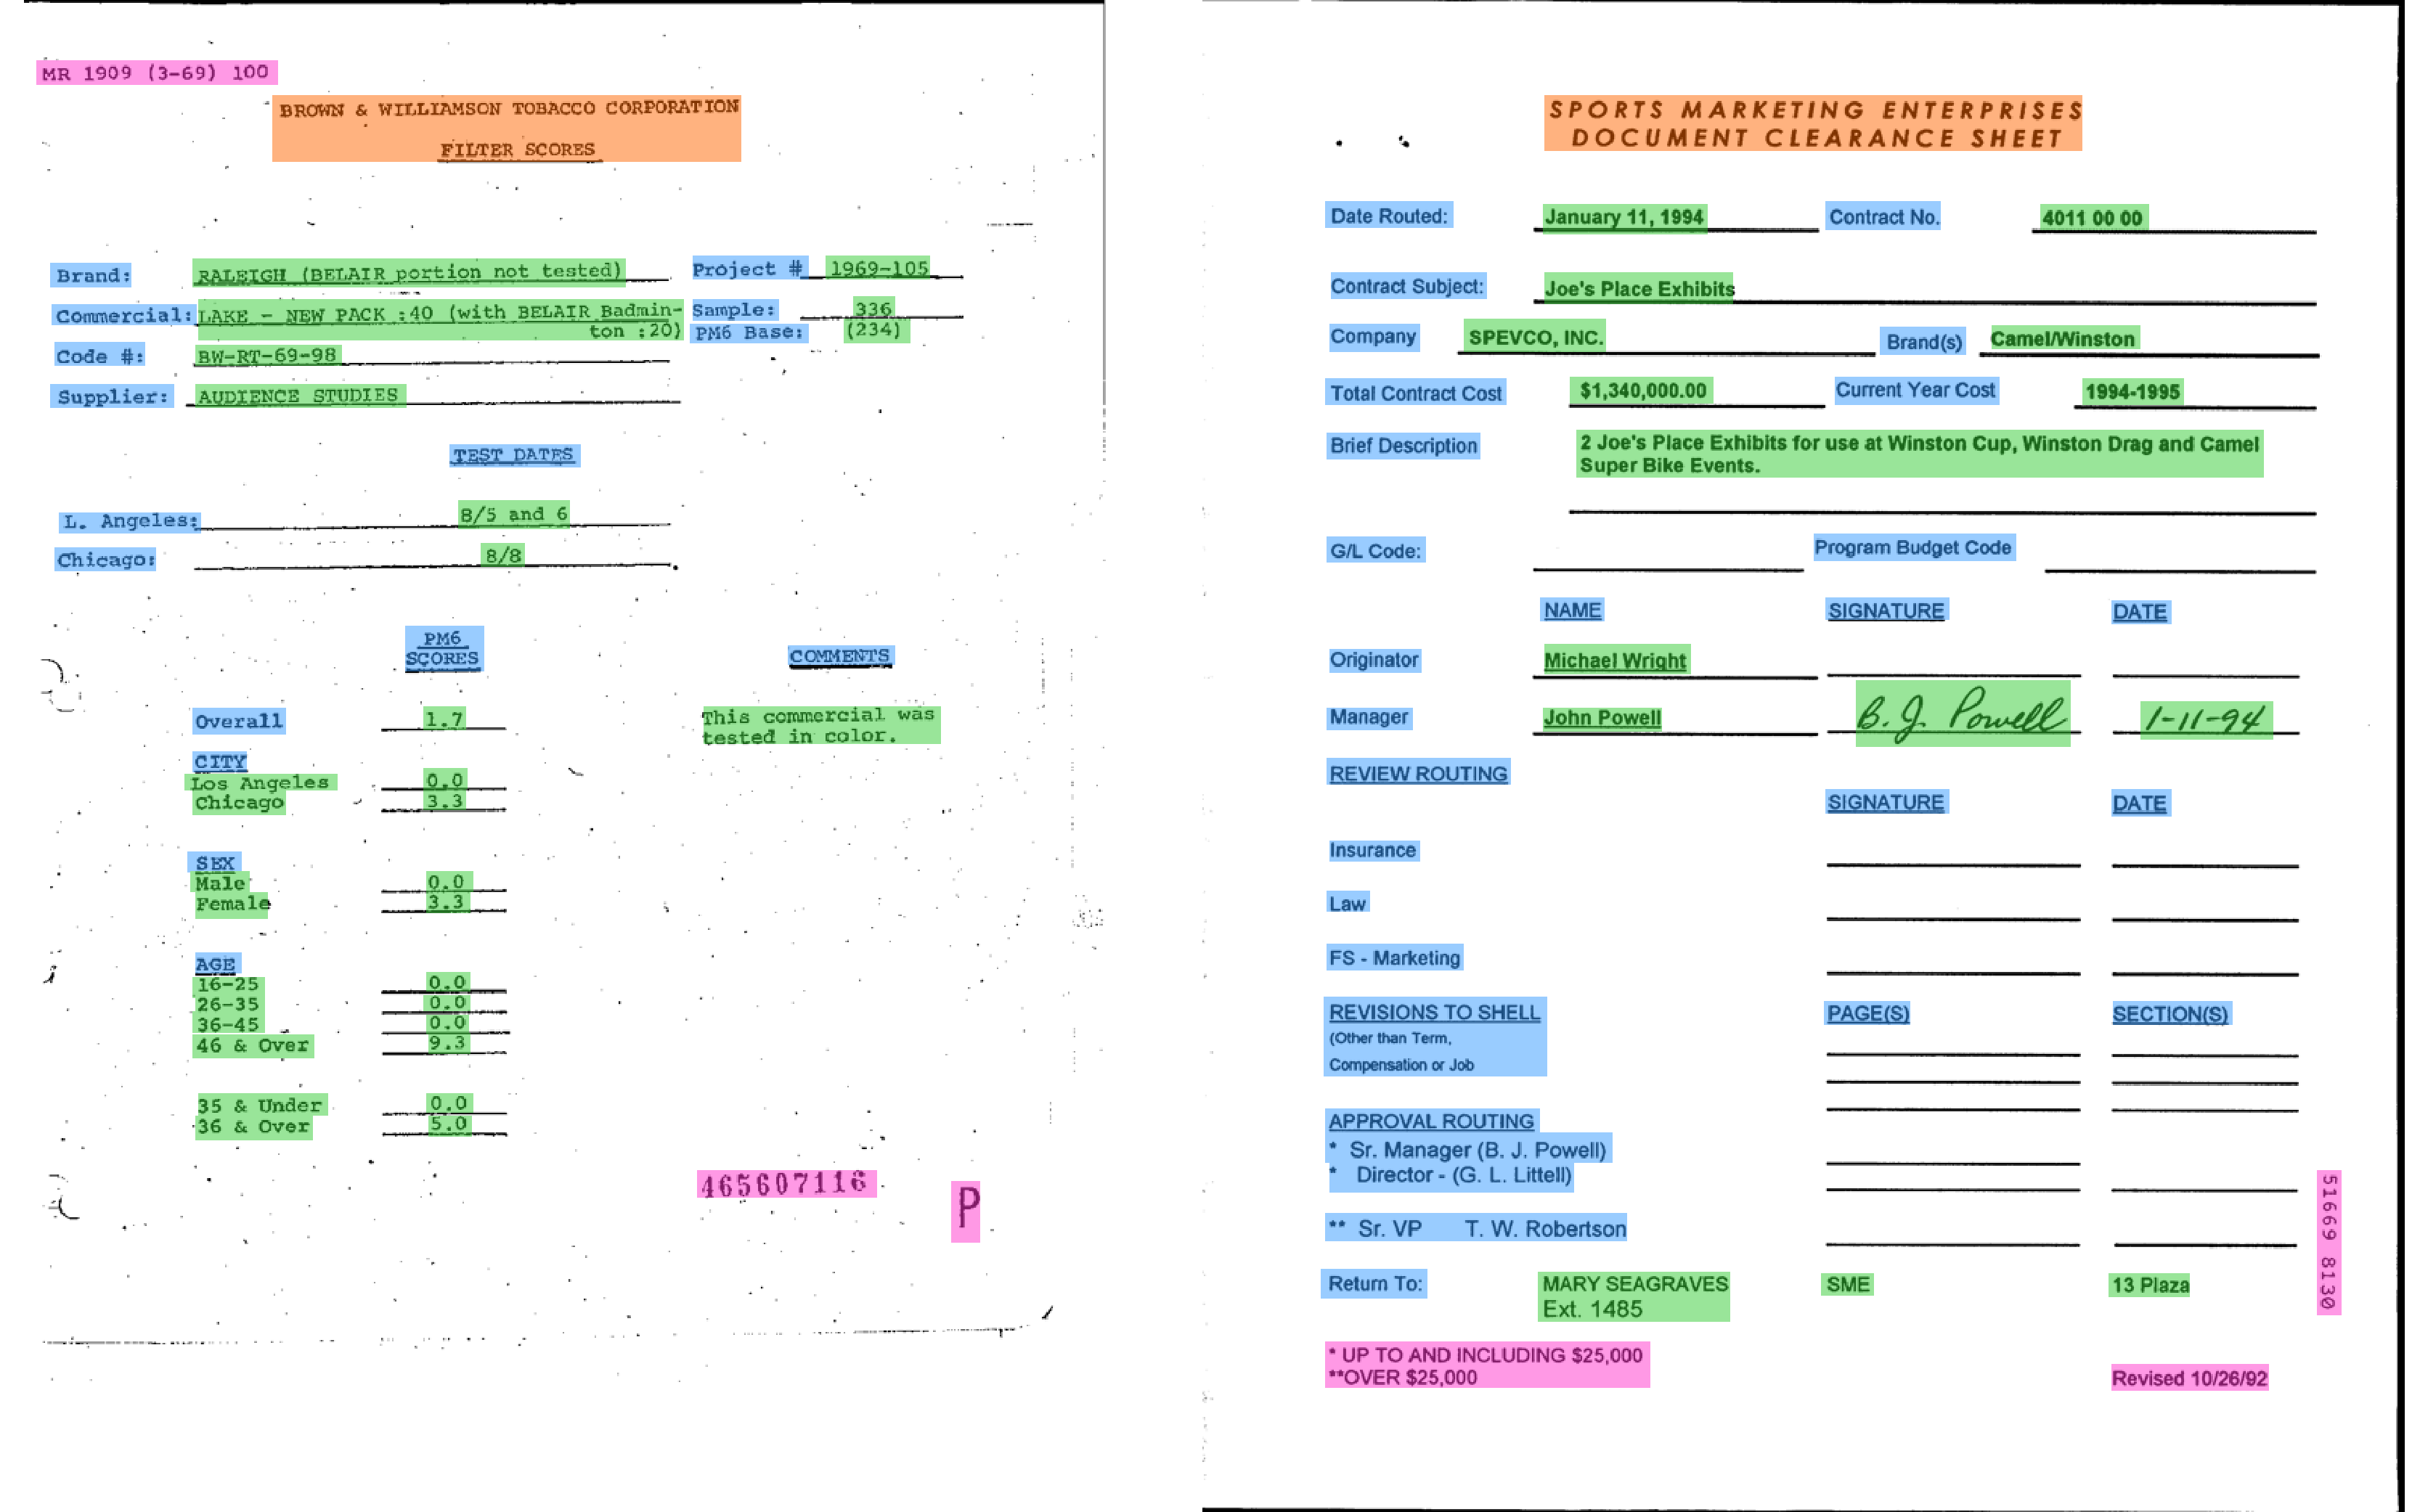
\includegraphics[width=\textwidth]{images/chapter2/two_forms.pdf}
%     \caption{Examples from FUNSD. Best viewed in color. Source: \url{https://guillaumejaume.github.io/FUNSD/}.}
%     \label{fig:examples-funsd}
%   \end{figure}
  

\textit{Visual information extraction} consists in extracting semantic \textit{entities} (\textit{entity recognition}) and their relationships (\textit{relation extraction}) from visually-rich documents, based on a set of pre-defined \textit{keys}. In contrast to traditional text-only information extraction, the two-dimensional spatial arrangement of text requires an understanding of page layouts for complete comprehension. 

Notable public datasets for this task include \ac{FUNSD} \citep{jaume2019funsd}, a form understanding dataset consisting of 199 real, noisy, and fully annotated scanned forms. These forms are organized as a list of interlinked form entities. Each semantic entity is characterized by a unique identifier, an entity type (\textit{i.e.}, key), a list of links with other entities, and a list of words and their corresponding bounding boxes. The dataset features three keys for which values need to be extracted: question, answer, and header. For receipt understanding, \ac{SROIE} \citep{huang2019icdar2019} (973 English documents) and \ac{CORD} \citep{park2019cord} (1000 Indonesian documents) are widely used datasets. In \ac{SROIE}, every receipt is formatted as a list of text lines, with each line being associated with word bounding boxes. The receipts are classified into four entity types: company, date, address, and total. In \ac{CORD}, receipts are arranged as lists of entities, each identified by a unique identifier, an entity type, and a list of words along with their respective bounding boxes. \ac{CORD} encompasses 30 entity types, further categorized into four superclasses: menu, subtotal, total, and void. In Chapter~\ref{chapter:layout2pos}, we employ these datasets to evaluate our work for visual information extraction tasks.

Several datasets have been proposed to advance entity extraction from more complex documents. Kleister \citep{gralinski2020kleister} comprises non-disclosure agreements and financial reports, typically characterized by their extensive length. The DeepForm dataset provided by \citet{borchmann2021due} is an improved version of the original dataset\footnote{\url{https://wandb.ai/stacey/deepform_v1}} featuring advertising disclosure forms with manually corrected invalid data points. Additionally, the PWC dataset, also proposed by \citet{borchmann2021due}, reformulates the original PWC Leaderboards dataset \citep{kardas2020axcell} into a visual information extraction task, using digital-born scientific papers as input instead of tables. VRDU-Registration Forms and VRDU-Ad-buy Forms \citep{wang2023vrdu} contain public documents downloaded from the Foreign Agents Registration Act\footnote{\url{https://www.justice.gov/nsd-fara}} and the Federal Communications Commission,\footnote{\url{https://publicfiles.fcc.gov/}} respectively. Three settings of increasing difficulty have been introduced to evaluate the model's performance across diverse scenarios. These scenarios range from handling a single template across training, validation, and testing, to the conventional setting where all three sets contain documents from the same template set, and finally, to the challenging scenario where documents in the sets are drawn from distinct template sets. 

To prompt further research into multilingual document understanding systems, datasets for visual information extraction containing documents in languages other than English have been proposed. EPHOIE \citep{wang2021towards} contains Chinese document images collected from scanned examination papers. XFUND is a multilingual extension of \ac{FUNSD} \citep{xu-etal-2022-xfund} and contains manually-labeled forms in 7 languages.

% Visual information extraction tasks can be framed as a Computer Vision problem, where semantically meaningful regions are detected through text box detection, and labeled using semantic segmentation. 

% Given a document and a set of keys, Key Information Extraction consists in extracting from the document the values of the given set of keys, e.g., the total amount in a receipt or the date in a form. In \ac{KIE} tasks, documents have a layout structure that is crucial for their interpretation. Notable public datasets in the field include the FUNSD (Form Understanding in Noisy Scanned Documents) dataset \citep{jaume2019funsd}, consisting of 199 real, noisy and fully annotated scanned forms. For receipt understanding, SROIE (Scanned Receipts OCR And Key Information Extraction) \citep{huang2019icdar2019} (973 documents) and CORD (Consolidated Receipt Dataset) \citep{park2019cord} (1000 documents) are widely used. \citet{gralinski2020kleister} elicit progress on deeper and more complex \ac{KIE} by introducing Kleister-NDA and Kleister-Charity, two collections of, respectively, non-disclosure agreements and financial reports with varying lengths. The objective is to help extending the understanding of documents with substantial lengths, various reasoning problems, complex layouts and OCR quality problems.


\subsection{Document Visual Question Answering}

% processing the multimodal information (\textit{i.e.}, text, layout, images) conveyed by the document

\textit{Document visual question answering} is a high-level understanding task that requires providing the correct answer to a question related to a visually-rich document, posed in natural language. This is achieved by jointly reasoning over the document layout (page structure, forms, tables), textual content (handwritten or typewritten), and visual elements (marks, tick boxes, diagrams). Unlike traditional visual question answering tasks, textual information holds a pivotal role in document visual question answering. The DocVQA dataset \citep{mathew2021docvqa} contains more than 12,000 industry documents and 5,000 corresponding questions. InfographicsVQA \citep{mathew2022infographicvqa} comprises infographic images with questions that require elementary reasoning and basic arithmetic skills. To spurr further research on developping generation abilities, VisualMRC \citep{tanaka2021visualmrc} was built from multiple domains of webpages and requires producing long and abstractive answers. For question answering over tables, \citet{borchmann2021due} converted the WikiTableQuestions dataset \citep{pasupat2015compositional} into a document visual question answering dataset by using HTML tables sourced from Wikipedia as input, in place of the original semi-structured HTML tables. \\

% Document \ac{VQA} can be approached in different ways, depending on the characteristics of the dataset. In the case of the DocVQA dataset, where answers to questions often take the form of text fragments within the document, prevailing methods model the problem as a machine reading comprehension task. In this scenario, the model is provided with visual features and textual contents and is tasked with extracting relevant text fragments from the documents based on the questions. In contrast, for datasets like VisualMRC, answers usually do not appear in the document as text fragments, and a longer abstractive answer is required. An effective strategy for such cases involves using a text generation method to generate answers to the questions. 

\subsection{Towards Advancing Document Understanding}

The number of open-sourced benchmark datasets proposed for these tasks has significantly facilitated the development of new techniques and models. Particularly noteworthy is the recent surge in deep learning-based models that have achieve state-of-the-art performance across these tasks. In line with the aforementioned works, we introduce novel datasets for layout-aware summarization—a task that has received limited attention in the document understanding field—in Chapter~\ref{chapter:loralay}. 

% Particularly noteworthy is the recent surge in deep learning-based models that have achieve state-of-the-art performance across these tasks.

% \section{Deep Learning-based Document Understanding}

\section{Task-specific Deep Learning Models For Document Understanding}

Deep Learning marked a paradigm shift by enabling significant performance leaps across various research areas. In particular, the fields of \ac{NLP} and Computer Vision have undergone substantial advancements due to the emergence of Deep Learning. The development of Document Understanding also reflects a similar trend, where methodologies from \ac{NLP} and Computer Vision are integrated into modern document understanding systems. 

The initial approach to enhancing document understanding system with Deep Learning involves the use of task-specific methods. These methods leverage pre-trained Computer Vision and/or \ac{NLP} models to gather knowledge from the corresponding modality. Features are extracted from either a single modality or through a simple combination of modality features, and used for a specific downstream task. 

% We first explore the early application of Deep Learning to improve Document Understanding, focusing on task-specific methods. We then delve into the more recent and successful strategy based on general-purpose multimodal pre-training. Drawing inspiration from \ac{BERT} and other foundation models, layout/visually-aware language models are pre-trained on extensive corpora and fine-tuned across a variety of document understanding tasks.

%  but the success of Deep Learning has put Computer Vision and \ac{NLP} models at the heart of contemporary approaches.

% \subsection{Task-specific Deep Learning Models}

\subsection{Document Image Classification} 

Document image classification constitutes a subtask of image classification. Consequently, classification models originally designed for natural images can be applied to tackle the challenges associated with document image classification. \citet{afzal2015deepdocclassifier} used a deep \ac{CNN} trained on the millions of examples from ImageNet \citep{deng2009imagenet}. \citet{das2018document} introduced a range of deep \acp{CNN} designed to classify specific regions within a document. These classifiers are combined using an effective ensembling technique for document image classification. \citet{dauphinee2019modular}  developed a model consisting of two distinct components — one dedicated to processing text and the other to handling images. This modular approach uses both visual information and textual content within a page to classify document images.

\subsection{Document Layout Analysis} 

Document layout analysis can be framed as an instance segmentation task for document images, where units such as text, figures, headings, paragraphs, and captions are the objects that need to be detected and recognized. For this task, the model has to predict per-pixel labels to categorize regions of interest within the document. Framing document layout analysis as an instance segmentation task offers flexibility and can adapt to both the coarser-grained task of page segmentation and the finer-grained task of logical structural analysis. Most deep learning based document layout analysis borrow various \ac{CNN}-based object detection and segmentation frameworks \citet{ren2015faster, cai2018cascade}. \citet{yang2017learning} proposed an end-to-end \ac{CNN} that combines both text and visual features within an encoder-decoder architecture for pixel classification. The encoder-decoder architecture ensures that visual feature information at various levels of resolution is considered throughout the encoding and decoding process \citep{burt1987laplacian}. In addition to the resulting visual representation, text embeddings learned from a pre-trained \ac{NLP} model are supplied at the final decoding layer. Similarly, \citet{oliveira2018dhsegment} introduced a multi-task pixel-by-pixel prediction \ac{CNN}-based model to perform layout analysis on historical documents. \citet{soto2019visual} view layout analysis of scientific articles as an object detection task. While instance segmentation requires delineating the boundaries of individual instances at the pixel level, object detection primarily focuses on identifying and locating objects using bounding boxes. \citet{soto2019visual} find that integrating contextual information into Faster R-CNN \citep{ren2015faster}, a prominent object detection framework, leverages local invariance of article elements and improves region detection performance. 

Faster R-CNN has been particularly successful when directly applied to table detection, a task often framed as an object detection task. CascadeTabNet \citep{prasad2020cascadetabnet} leverages the Cascade R-CNN \citep{cai2018cascade} model for simultaneous table detection and table structure recognition. Another notable contribution is TableSense \citep{dong2019tablesense}, which significantly enhances table detection by introducing cell features and employing advanced sampling algorithms. 

Most deep learning based document layout analysis and table understanding models mainly focus on processing visual features of layout components using \ac{CNN}-based models. Visual features alone may fall short in solving document layout analysis tasks due to their limited ability to capture underlying semantics, structural relationships, and textual content. For better layout analysis, it is crucial to integrate both visual and semantic information while capturing and encoding relationships between layout components \citep{luo2022doc}. We explore this direction in Chapter~\ref{chapter:skim-attention}.


\subsection{Visual Information Extraction} 

For information extraction from visually-rich documents, many researchers and practitioners have framed the problem as an instance segmentation task. In this approach, semantically meaningful regions are identified through object detection and labeled via semantic segmentation. Given the pivotal role of text in visual information extraction, directly embedding textual information into the image simplifies handling of 2D textual relationships. The conventional framework considers document images as a pixel grid of dimensions $w \times h \times d$, where $w$ is the image width, $h$ is the image height, and $d$ is the text embedding dimension. In this grid, each pixel corresponds to a text embedding vector, preserving the layout of documents and capturing details such as positioning, size, and alignment for textual components. As an initial attempt, Chargrid \citep{katti2018chargrid} operates at the character level, using a one-hot encoding for each character. A 2D grid of characters is constructed by mapping each pixel intersecting with a character bounding box to the corresponding one-hot encoding. A convolution-based encoder-decoder model is then applied to perform instance-level segmentation. Specifically, the model predicts a segmentation mask where each pixel is assigned a class label, and generates object bounding boxes to assign characters from the same segmentation class to distinct instances. Expanding on Chargrid, VisualWordgrid \citep{kerroumi2021visualwordgrid} operates at the word level, incorporating word embeddings from Word2Vec or fastText. To improve the end-to-end accuracy, BERTgrid \citep{denk2019bertgrid} constructs a grid at the word-piece level, embedding each word piece with dense contextualized vectors obtained from \ac{BERT}. ViBERTgrid \citep{lin2021vibertgrid} takes a step further by concatenating a BERTgrid to an intermediate layer of a \ac{CNN} model, resulting in a more powerful grid-based document representation. 

Documents can also be represented as graphs, wherein nodes correspond to textual segments, and relationships between text fragments are modeled as edges. \citet{liu2019graph} introduce a model based on \acp{GCN} to integrate both textual and visual information. In this model, each node comprises information about the position of the segment and the text it contains, while edges represent the relative distances between the corresponding segments and their aspect ratio. Graph convolution is employed to calculate graph embeddings for each text segment, which are then combined with text embeddings. The resulting embeddings are fed into a bidirectional \ac{LSTM} for information extraction from in-house invoices and receipts. This graph-based approach ensures that both local and global information can be learned. \citet{hwang2020spatial} model a document as a directed graph, extracting information through dependency analysis. \citet{yu2021pick} combines graph learning with graph convolution to achieve richer semantic representations.

In Chapter~\ref{chapter:layout2pos}, we tackle visual information extraction tasks through a distinct approach, leveraging general-purpose multimodal pre-training methods for a broader and more versatile perspective.

% \subsubsection{Document Visual Question Answering} 

% Document visual question answering an be approached in different ways, depending on the characteristics of the dataset. In the case of the DocVQA dataset, where answers to questions often take the form of text fragments within the document, prevailing methods model the problem as a machine reading comprehension task. In this scenario, the model is tasked with extracting relevant text fragments from the documents based on the questions. \citet{mathew2021docvqa} showed that BERT outperforms state-of-the-art text-augmented \ac{VQA} models \citep{singh2019towards, hu2020iterative} on DocVQA. In contrast, for datasets like VisualMRC, answers usually do not appear in the document as text fragments, and a longer abstractive answer is required. An effective strategy for such cases involves using a text generation method to generate answers to the questions. \citet{tanaka2021visualmrc} extended BART and T5 with bounding box information and layout features.

% However, these models are all designed for specific tasks and document types. Because the domain knowledge of one document type cannot be easily transferred into another, the models have to be re-trained when the document type is changed. Hereby, models based on shallow fusion cannot fully exploit the layout invariance among different document types (e.g. the arrangement of key-value pairs in forms is usually in the left-right order or the top-down order). Additionally, they rely on labeled data, yet many tasks related to Document Understanding are label-scarce. Following the current research trend in \ac{NLP}, a framework that can learn from unlabeled documents through pre-training and perform model fine-tuning for specific downstream applications is preferred over ones that require fully-annotated training data.


\section{Deep Fusion of Modalities via General-purpose Multimodal Pre-training}
\label{section:related-document-understanding-deep-fusion}

While the aforementioned methods demonstrate good performance across document understanding tasks, they still face significant limitations. The majority of these models are all designed for specific tasks and document types. As such, these approaches rely on labeled data; however, most datasets related to Document Understanding are label-scarce. This scarcity arises from the labor-intensive and time-consuming nature of the human annotation process. Driven by data limitations, these task-specific models often rely solely on pre-trained Computer vision models and/or \ac{NLP} models, each trained independently. A common practice involves combining the knowledge gained from each modality through a shallow fusion of features, such as concatenation. However, this approach makes it challenging to easily transfer domain knowledge from one document type to another. This stems from the need to re-train models from scratch when the document type is changed.

% However, the correlation between different tasks, such as shared semantic representations between visual information extraction and document visual question answering, cannot be effectively leveraged. This stems from the need to re-train models from scratch when changing tasks, as the domain knowledge specific to one task cannot be easily transferred to another. 

% which cannot fully exploit the layout invariance among different document types (\textit{e.g.}, the arrangement of key-value pairs in forms is usually in the left-right order or the top-down order). This stems from the necessity of re-training models when the document type is changed. This is because the domain knowledge specific to one document type cannot be easily transferred to another. 

Visually-rich documents encompass three modalities that inherently align: text, layout, and visual information. Layout, \textit{i.e.}, the spatial relationship of text blocks within a document, facilitates reading comprehension and information searching \citep{meyer1980use, guthrie1991roles, wright1999psychology}. For instance, the arrangement of key-value pairs in forms typically follows a left-right or top-down order. In addition to spatial information, the visual elements presented with the text can offer global structural information (\textit{e.g.} there is a clear visual distinction between different document types) and help with downstream tasks (\textit{e.g.}, the title of documents is usually enlarged). Hence, it becomes vital to jointly learn text with layout and visual information.

As visually-rich documents are widely used in real-world applications, there is a substantial volume of unlabeled documents. This provides an opportunity for leveraging self-supervised pre-training methods. The widespread success and popularity of pre-training techniques, notably those employing the Transformer architecture \citep{vaswani2017attention}, emphasize the critical role of deep contextualization for sequence modeling in both \ac{NLP} and Computer Vision problems. Following the current research trend, a general-purpose framework that can learn from unlabeled documents through pre-training and perform model fine-tuning for different types of downstream applications is preferred over ones that are task-specififc and require fully-annotated training data. This trend has prompted a shift in Document Understanding towards the "pre-training then fine-tuning" paradigm, establishing pre-training techniques as the \textit{de facto} approach in the field over years. In particular, researchers and practitioners have been leveraging the Transformer architecture to attain cross-modal alignment via joint pre-training of text, layout, and images from large amounts of unlabeled data. This approach enables pre-trained models to absorb cross-modal knowledge across various document types. Consequently, when the model is applied to a different domain with different document formats, only a small number of labeled samples are required to fine-tune the generalized model effectively. 

Next, we discuss general-purpose, multimodal pre-training methods for Document Understanding. We review these methods from several viewpoints, considering the various challenges in the field. This includes the integration of layout, image encoding, the pre-training tasks used, the incorporation of positional information, model initialization, and considerations for multilingual and long-range aspects. 

The models discussed are summarized in Table~\ref{table:document-understanding-models}. Through pre-training, these models have learned general representations that can be fine-tuned for a wide range of tasks. Notably, these pre-trained models demonstrate remarkable performance, surpassing state-of-the-art task-specific models across document image classification \citep{xu2020layoutlmv2}, information extraction \citep{peng2022ernie}, and document layout analysis \citep{li2020docbank} tasks. In parallel with the development of datasets for document visual question answering, the use of self-supervised pre-training methods has yielded notable achievements in the corresponding tasks \citep{appalaraju2021docformer, tanaka2021visualmrc}. 

% Hence, integrating layout and visual information into the pre-training stage allows for cross-modal alignment via self-supervised, joinHence, layout and visual information can be integrated into the pre-training stage to be jointly learned alongside the text. In particular, researchers and practitioners have been leveraging the Transformer architecture to attain cross-modal alignment via self-supervised, joint multimodal pre-training from large amounts of unlabeled data.

\begin{table}[h]
\centering
\small
\begin{adjustbox}{max width=\textwidth}
\renewcommand{\arraystretch}{1.25}
\begin{threeparttable}
\begin{tabular}{lcccccccc}
    \toprule
        & \textbf{Architecture} &                           & & \multicolumn{3}{c}{\textbf{Layout}} \\            
        & & \textbf{Visual Encoding}  & & \textbf{Bounding Box}  & \textbf{Encoding} & \textbf{Relative Bias} \\
        & & & & \textbf{Granularity} & & \\
    \midrule
    \rowcolor{lightgray}
    LayoutLM \citep{xu2020layoutlm} & Encoder & \xmark & & Word & Embedding Tables & \xmark \\
    LayoutLMv2 \citep{xu2020layoutlmv2} & Encoder & ResNeXt-FPN & & Word & Embedding Tables & \cmark \\
    \rowcolor{lightgray}
    LayoutXLM \citep{xu-etal-2022-xfund} & Encoder & ResNeXt-FPN & & Word & Embedding Tables & \cmark \\
    LayoutLMv3 \citep{huang2022layoutlmv3} & Encoder & Embedding Tables & & Block & Embedding Tables & \cmark \\
    \rowcolor{lightgray}
    \citet{pramanik2020towards} & Encoder & ResNet50-FPN & & Word & Embedding Tables & \xmark \\
    DocFormer \citep{appalaraju2021docformer} & Encoder & ResNet50 & & Word & Embedding Tables & \xmark \\
    \rowcolor{lightgray}
    ERNIE-Layout \citep{peng2022ernie} & Encoder & ResNeXt-FPN & & Word & Embedding Tables & \cmark  \\
    FormNet \citep{lee2022formnet} & Encoder & \xmark & & Word & \xmark & \cmark \\
    \rowcolor{lightgray}
    BROS \citep{hong2020bros} & Encoder & \xmark & & Word & Sinusoidal functions & \xmark \\
    StructuralLM \citep{li2021structurallm} & Encoder & \xmark & & Block & Embedding Tables & \xmark \\
    \rowcolor{lightgray}
    SelfDoc \citep{li2021selfdoc} & Dual-stream encoder & Faster R-CNN & & Block & \xmark & \xmark \\ 
    LiLT \citep{wang2022lilt} & Dual-stream encoder & \xmark & & Word & Embedding Tables & \xmark \\
    \rowcolor{lightgray} 
    % DiT \citep{li2022dit} & Encoder + detection framework & Embedding Tables & & \xmark & \xmark & \xmark \\
    H-VILA \citep{shen2022vila} & Hierarchical encoder & \xmark & & Block & Embedding Tables & \xmark \\ 
    \rowcolor{lightgray}
    LAMPreT \citep{wu2021lampret} & Hierarchical encoder & CNN + Linear Layer & & Block & \xmark & \xmark \\
    TILT \citep{powalski2021going} & Encoder-decoder & U-Net & & Word &\xmark & \cmark \\
    \rowcolor{lightgray}
    LayoutT5 \citep{tanaka2021visualmrc} & Encoder-decoder & Faster R-CNN & & Word & Embedding Tables & \xmark \\
    LayoutBART \citep{tanaka2021visualmrc} & Encoder-decoder & Faster R-CNN & & Word & Embedding Tables & \xmark \\
    \rowcolor{lightgray}
    Donut \citep{kim2022ocr} & Encoder-decoder & Swin Transformer & & \xmark & \xmark & \xmark \\
\bottomrule
\end{tabular}
\end{threeparttable}
\end{adjustbox}
\caption{Summary of general-purpose, multimodal pre-training document understanding models.}
\label{table:document-understanding-models}
\end{table}

% On RVL-CDIP, LayoutLM outperforms several state-of-the-art convolution-based baselines.For document layout analysis, \citet{li2020docbank} show that LayoutLM model significantly outperforms Faster R-CNN on the DocBank dataset.

\subsection{Representing Layout-rich Documents}

The layout of a document defines its visual structure. Effectively incorporating layout information provides valuable cues for accurate interpretation and organization of information, addressing the challenges posed by complex and varied document layouts in document understanding tasks. We explore strategies for incorporating layout information into Transformer models, delving into layout encodings and layout-aware model architectures. Then, we focus on modifications to the attention mechanism that explicitly include layout information. Finally, we examine the role of position encodings in the context of document understanding tasks, where complex layouts and potential reading order inaccuracies pose significant challenges.

\subsubsection{Incorporating Layout Information} 

As the first work to jointly learn text and layout information, LayoutLM \citep{xu2020layoutlm} stands out as the pioneer work in multimodal pre-training for document understanding tasks. Over time, it has become the building block for designing more complex document understanding sytems. LayoutLM encodes layout information with learned 2D position embeddings. A 2D position embedding carries information about the spatial position of a token within the document page. The spatial position of a token is represented by its bounding box $(x_0, y_0, x_1, y_1)$ obtained by an \ac{OCR} engine \citep{kay2007tesseract}, where $(x_0, y_0)$ and $(x_1, y_1)$ respectively denote the upper-left and lower-right corners. The coordinates are discretized and normalized to integers in $[0, \ldots, 1000]$. Four embedding tables are used to encode spatial positions: two for the coordinates axes ($x$ and $y$) and the other two for the bounding box size (width and height). The final layout embedding $\bell \in \mathbb{R}^{d_{\ell}}$, for a token located at position $(x_0, y_0, x_1, y_1)$, is defined by:

\begin{equation}
\begin{split}
    \bell & = \text{2DPosEmb}_x(x_0) + \text{2DPosEmb}_y(y_0) \\
    & + \text{2DPosEmb}_x(x_1) + \text{2DPosEmb}_y(y_1) \\
    & + \text{2DPosEmb}_w(x_1 - x_0) \\
    & + \text{2DPosEmb}_h(y_1 - y_0) \\
\end{split}
\end{equation}

\noindent These 2D position embeddings are added to the sequential position and text embeddings of \ac{BERT}. The resulting input sequence is passed through an encoder similar to \ac{BERT}. Via the self-attention mechanism, encoding 2D position features into the language model improves alignment between layout information and semantic representation. 

Building on the groundwork laid by LayoutLM, many works have introduced alternative approaches to encode layout information. BROS \citep{hong2020bros} employs sinusoidal functions as an alternative to linear embedding layers to encode continuous values for the spatial positions of tokens on the page. In addition to spatial positions, DocFormer \citep{appalaraju2021docformer} incorporates the Euclidean distance from each corner of a bounding box to the corresponding corner in the bounding box to its right, as well as the distance between centroids of the bounding boxes. DocFormer, as well as ERNIE-Layout \citep{peng2022ernie}, create separate layout features for visual and language modalities. Driven by the consideration that 2D dependencies might differ across layers, DocFormer introduces layout features as residual connections to each layer of a Transformer encoder, as opposed to directly adding them to language features. In addition, layout features are shared across modalities to enforce feature correlation across modalities. 

Based on the assumption that words in a block typically convey the same semantic meaning, certain studies favor leveraging information from content blocks (such as header, paragraph, figure) rather than operating at the word level, as contextualization between every word may be redundant and overlook localized context. StructuralLM \citep{li2021structurallm} departs from word-level 2D positions and leverages block-level 2D positions derived from the bounding boxes obtained through \ac{OCR}. As such, words that belong to the same block share the same 2D position embeddings. This approach allows the model to discern which words belong to the same block, thereby enhancing contextual representations of cells. Similarly, LayoutLMv3 \citep{huang2022layoutlmv3} models the layout information of blocks by adopting block-level 2D positions.

% In \ac{LAMPreT} \citep{wu2021\ac{LAMPreT}}, the layout is obtained by parsing a document into content blocks, each being assigned a block position, a block type (\textit{e.g.}, header, paragraph, image), and block attributes (\textit{i.e.}, font size, boldness, underline, and italic appearance). The document layout is defined as the structural presentation of the content blocks, and the aforementioned features of the textual contents within a block. 

Rather than treating layout information as an additional feature, some research works have modified model architectures to align with the specific layout formulation of documents. In \ac{LAMPreT} \citep{wu2021lampret}, the layout is obtained by parsing a document into content blocks using PDF parsing tools. The layout is then defined as the structural presentation of these content blocks, and processed by two cascaded Transformers. The first one deals with the contents of a block, while the second one focuses on how these blocks are spatially structured. SelfDoc \citep{li2021selfdoc} uses the visual features of content blocks obtained with an object detection model, Faster R-CNN \citep{ren2015faster}, trained on semantically meaningful components such as text blocks, titles, lists, tables, and figures. H-VILA \citep{shen2022vila} parses the document to extract group of tokens, which are then encoded using a hierarchical Transformer. For visual information extraction tasks, Token Path Prediction \citep{zhang2023reading} models the document layout as a complete directed graph of tokens. UDOP \citep{tang2023unifying} fuses image pixels and text tokens based on layout information, \textit{i.e.}, the input representation of a token is the sum of its text representation and the image feature of the patch  to which it belongs. Our approach in Chapter~\ref{chapter:skim-attention} is in line with the concept of adapting model architectures to suit the layout formulation of documents. Building on prior works in cognitive sciences, we introduce a novel attention mechanism that relies solely on the spatial positions of tokens in the page. This approach mirrors the human process of skimming through a document to extract its inherent structure.


\subsubsection{Layout-aware Attention Mechanisms}
\label{section:related-document-understanding-layout-aware-attention}

The order two tokens are in, how many tokens separate them, or how many pixels apart they are, are often relevant to the decision of how strongly a token should attend to another one. However, 2D position embeddings can only implicitly capture the relationship between tokens within a document. To address this limitation and effectively model local invariance in document layout, various research works have introduced advanced approaches to integrate layout information by incorporating the spatial relationships between tokens directly into the attention calculation process.

Extending the concept of 1D relative position bias \citep{raffel2020exploring} to the 2D scenario, LayoutLMv2 \citep{xu2020layoutlmv2} builds upon LayoutLM by incorporating \textit{bias} terms that encode the 2D relative position of tokens with respect to each other. These bias terms are added to the attention scores to explicitly capture the relationship between tokens, defining a \textit{spatial-aware attention mechanism}. Formally, the pre-softmax attention scores are defined as follows:

\begin{equation}
    \alpha_{i,j} = \dfrac{1}{\sqrt{d}} \bm{q}_i \cdot \bm{k}_j + \bm{b}^{(1D)}_{j - i} + \bm{b}^{(2D_x)}_{x_j - x_i} + \bm{b}^{(2D_y)}_{y_j - y_i},
\end{equation}

\noindent where $\bm{b}^{(1D)}$, $\bm{b}^{(2D_x)}$, and $\bm{b}^{(2D_y)}$ correspond to the sequential, horizontal, and vertical relative position biases, respectively. Likewise, TILT \citep{powalski2021going} incorporates 2D relative positions while entirely discarding the use of absolute 2D positions in its encoding strategy. 

To introduce a spatial perspective to the computation of semantic similarity within attention, both DocFormer \citep{appalaraju2021docformer} and ERNIE-Layout \citep{peng2022ernie} decouple attention into distinct components. 
ERNIE-Layout uses a disentangled attention mechanism \citep{he2020deberta}. In this mechanism, each token is represented using four sets of query-key-value, with each set encoding the token's content (\textit{i.e.}, text and image), relative sequential positions ($1D$), relative horizontal positions ($2D_x$), or relative vertical positions ($2D_y$). Attention\footnote{For the sake of clarity, we omit the scaling and softmax operations.} between two tokens is computed as the sum of standard (\textit{i.e.}, content-based) attention and the following components: 

\begin{equation}
        \alpha^{\star}_{ij} = \bm{q}_i \cdot {\bm{k}^{\star}_{\delta_{\star}(i, j)}}^{\top} + \bm{k}_j \cdot {\bm{q}^{\star}_{\delta_{\star}(j, i)}}^{\top}, \qquad \forall \text{ } \star \in \{1D, 2D_x, 2D_y\}
\label{equation:ernie-layout-attention}
\end{equation}

% Attention\footnote{For the sake of clarity, we omit the scaling and softmax operations.} between two tokens is computed as the sum of standard (\textit{i.e.}, content-based) attention and the following components:

% \begin{equation}
%     \begin{aligned}
%         \alpha^{(1D)}_{ij} &= \bm{q}_i \cdot {\bm{k}^{(1D)}_{\delta(i, j)}}^{\top} + \bm{k}_j  \cdot {\bm{q}^{(1D)}_{\delta(j, i)}}^{\top} \\
%         \alpha^{(x)}_{ij} &= \bm{q}_i \cdot {\bm{k}^{(x)}_{\delta_x(i, j)}}^{\top} + \bm{k}_j  \cdot {\bm{q}^{(x)}_{\delta_x(j, i)}}^{\top} \\
%         \alpha^{(y)}_{ij} &= \bm{q}_i \cdot {\bm{k}^{(y)}_{\delta_y(i, j)}}^{\top} + \bm{k}_j  \cdot {\bm{q}^{(y)}_{\delta_y(j, i)}}^{\top}, \\
% \end{aligned}
% \label{equation:ernie-layout-attention}
% \end{equation}
    
\noindent where relative positions $\delta_{\star}(i, j)$ are first mapped to relative position embeddings using embedding tables, then projected into query, key, and value vectors. Rather than using query-key-value projections, DocFormer directly incorporate relative position embeddings $\bm{b}^{(1D)}$ into its attention mechanism. Dismissing relative 2D positions, DocFormer defines attention as the sum of standard attention with 1D relative attention and layout-based attention, expressed as follows:

\begin{equation}
    \begin{aligned}
        \alpha^{(1D)}_{ij} &= \bm{q}_i \cdot \bm{b}^{(1D)}_{j-i} + \bm{q}_j \cdot \bm{b}^{(1D)}_{j-i} \\
        \alpha^{(2D)}_{ij} &= \bm{q}^{(2D)}_i \cdot \bm{k}^{(2D)}_j, \\
\end{aligned}
\label{equation:docformer-attention}
\end{equation}

\noindent where $\bm{q}^{(2D)}_i$ and $\bm{k}^{(2D)}_j$ are computed from the tokens' layout embeddings. 

% To prevent early merging of distinct types of relative (sequential and spatial) position information, ERNIE-Layout \citep{peng2022ernie} computes attention scores between tokens using \textit{disentangled} matrices on their semantics and relative sequential and spatial positions. Specifically, attention scores are disentangled into four components: language semantics (denoted by the subscript $S$), relative sequential positions ($1D$), relative horizontal positions ($x$), and relative vertical positions ($y$). Let $\delta_{1D}$, $\delta_x$, and $\delta_y$ be the sequential, horizontal, and vertical relative distance matrices between every pair of tokens in the sequence. Given the query and key projections $\bm{q}^\star, \bm{k}^\star$, where $\star \in \{s, 1D, x, y\}$, the disentangled unscaled pre-softmax attention scores are computed as follows:

% \begin{equation}
% \begin{aligned}
%     \alpha^{S}_{ij} &= \bm{q}^{S}_i \cdot \bm{k}^{S}_j \\
%     \alpha^{1D}_{ij} &= \bm{q}^{S}_i \cdot \bm{k}^{1D}_{\delta_{1D}(i, j)} + \bm{k}^{S}_j  \cdot \bm{q}^{1D}_{\delta_{1D}(j, i)} \\
%     \alpha^{x}_{ij} &= \bm{q}^{S}_i \cdot \bm{k}^{x}_{\delta_{x}(i, j)} + \bm{k}^{S}_j  \cdot \bm{q}^{x}_{\delta_{x}(j, i)} \\
%     \alpha^{y}_{ij} &= \bm{q}^{S}_i \cdot \bm{k}^{y}_{\delta_{y}(i, j)} + \bm{k}^{S}_j  \cdot \bm{q}^{y}_{\delta_{y}(j, i)} \\
% \end{aligned}
% \label{equation:ernie-layout-attention}
% \end{equation}

% \noindent These attention scores are summed up to get the final attention matrix.

% Similarly, DocFormer \citep{appalaraju2021docformer} modifies the self-attention mechanism to obtain spatially-aware features. In each Transformer layer, self-attention processes language semantics (denoted by $S$) and visual (denoted by $V$) modalities separately. Given $\star \in \{S, V\}$, let $\bell^{\star} = (\bell^{\star}_1, \ldots, \bell^{\star}_n)$ be the modality-specific layout features, and $\bm{q}^\star$, $\bm{k}^\star$, the query and key projections. Let $\bm{b}^{(1D)}$ represent the sequential relative position bias vector, and $\bm{W}^{(2D)}_q$ and $\bm{W}^{(2D)}_k$ be the learnable projection matrices for layout-specific query and key, respectively. The modality-specific attention score\footnote{For the sake of clarity, we omit the scaling and softmax operations.} for tokens $i$ and $j$ is disentangled as follows:

% \begin{equation}
%     \alpha^{\star}_{ij} = \left(\bm{q}^{\star}_i \cdot \bm{k}^{\star}_j\right) + \left(\bm{q}^{\star}_i \cdot \bm{W}^{(1D)}_{j-i}\right) + \left(\bm{q}^{\star}_j \cdot \bm{W}^{(1D)}_{j-i}\right) + \left(\bell^{\star}_i \cdot \bm{W}^{(2D)}_q \right) \left(\bell^{\star}_j \cdot \bm{W}^{(2D)}_k \right),
% \end{equation}

% \noindent where $\bm{W}^{(1D)}_{j-i}$ denotes the 1D relative position embedding between tokens $i$ and $j$.

% In SelfDoc \citep{li2021selfdoc}, self-attention in the cross-modal encoder is replaced by two cross-modal attention functions. The first function identifies the alignment between language and visual information, \textit{e.g.}, if the font size in a text is confirmed by the semantic meaning of language features, these features should be amplified. Let $\bm{q}^\star$, $\bm{k}^\star$, and $\bm{v}^\star$ denote the modality-specific query, key and value projections, where $\star \in \{S, V\}$. For the language modality, the first cross-modal attention function is defined as follows:

% \begin{equation}
%     f_{1}(\bm{q}^S_i, \bm{k}^V_j, \bm{v}^S_j) = \softmax \left( \dfrac{\bm{q}^S_i \cdot \bm{k}^V_j}{\sqrt{d}}\right) \bm{v}^S_j.
% \end{equation}

% \noindent The second attention function uncovers inner-relationships between modalities, \textit{e.g.}, similarity in font style between content blocks can improve the understanding of semantic meaning between these blocks. Formally:

% \begin{equation}
%     f_{2}(\bm{q}^V_i, \bm{k}^V_j, \bm{v}^S_j) = \softmax \left( \dfrac{\bm{q}^V_i \cdot \bm{k}^V_j}{\sqrt{d}}\right) \bm{v}^S_j.
% \end{equation}

% \noindent The vision modality undergoes the same process by swapping $S$ and $V$ in the above equations.

In \ac{LiLT} \citep{wang2022lilt}, text embeddings and layout embeddings are processed independently through separate encoders. To consider the cross-modal interactions between text and layout across the entire pipeline, a \textit{bidirectional attention complementation mechanism} is introduced. In each layer of the textual encoder, the attention scores are summed with those obtained by the layout encoder at the same layer, and vice-versa.   

Rather than using relative embeddings, FormNet \citep{lee2022formnet} incorporate features about relative positions by using trainable parametric functions coupled with error networks. For each feature type (\textit{e.g.}, the order of and log-distance between pairs of tokens), each pair of token representations is fed to the parametric function associated. The corresponding error network takes the observed (\textit{ground-truth}) feature and the output of the parametric function, and returns a penalty score that is subsequently added to the attention score. This process penalizes pairs whose predicted feature significantly deviates from the observed one.

% FormNet \citep{lee2022formnet} completely avoids the use of both absolute and relative (sequential and spatial) position embeddings. The underlying idea behind the attention mechanism in FormNet, Rich Attention, is that features such as the order two tokens are in, how many tokens separate them, or how many pixels apart they are, are often relevant to the decision of how strongly a token should attend to another one. Therefore, Rich Attention computes, for every pair of tokens, their order and log-distance with respect to the $x$ and $y$ axes on the grid. For an attention head at a certain layer $l$, the model computes the \textit{actual} \textit{order} $o_{ij}$ and \textit{log-distance} $o_{ij}$ between token representations $\bm{x}^{(l)}_i$ and $\bm{x}^{(l)}_j$:

% \begin{align}
%     o_{ij} &= \{i < j\} \\
%     d_{ij} &= \text{ln}(1 + \mid i - j \mid).
% \end{align}

% \noindent Using two affine functions $f^p$ and $f^{\mu}$, it then calculates the \textit{ideal} order $p_{ij}$ and log-distance $\mu_{ij}$ the tokens should have if there was a meaningful relationship between them:

% \begin{align}
%     p_{ij} &= \text{Sigmoid}\left(f^p(\bm{x}^{(l)}_i \mathbin\Vert \bm{x}^{(l)}_j)\right)\\
%     \mu_{ij} &= f^{\mu}(\bm{x}^{(l)}_i \mathbin\Vert \bm{x}^{(l)}_j).
% \end{align}

% \noindent The predicted and ground-truth orders and log-distances are then compared using binary cross-entropy and L2 loss functions, respectively. The corresponding losses are then added to the attention scores. By penalizing token pairs that violate these soft order/distance constraints, the ability to learn logicial implication rules is incorporated into the model.


\subsubsection{Incorporating Sequential Position Information}

All document pre-training techniques operate on serialized text. An \ac{OCR} engine or PDF parser is used to extract text from a document and serialize it according to a raster-scan order, which aligns tokens in a sequence from the top-left to the bottom-right corner. However, this arrangement does not always conform to human reading patterns, particularly for documents with complex layouts such as multicolumn texts, tables, and forms. This misalignment with human reading habits (\textit{i.e.}, \textit{serialization errors}) can result in suboptimal performance in document understanding tasks. 

To address this problem, automatic word reordering techniques can be employed. ERNIE-Layout \citep{peng2022ernie} uses an in-house document layout analysis toolkit that provides an appropriate reading order based on the spatial distribution of words, pictures, and tables. Enhanced with this knowledge, the token sequence can be rearranged in a way that yields a lower perplexity compared to the raster-scan order. This translates into a serialization that aligns better with human reading patterns. LayoutReader \citep{wang2021layoutreader} was designed to detect the reading order of documents and improve the line ordering capabilities of \ac{OCR} engines. This sequence-to-sequence model employs LayoutLM \citep{xu2020layoutlm} as its encoder, generating the reading order sequence for documents. Another strategy to mitigate reading order errors involves using more robust position encodings, as it has been shown that the performance of document Transformer models with learned positional embeddings significantly deteriorates on noisy data with incorrect reading order information \citep{hong2020bros}. \citet{wang2022simple} propose a \ac{LSPE} method based on feed-forward networks. Using sinusoidal functions enables the model to extrapolate to longer lengths not encountered during training. Simultaneously, the learnable feed-forward network component enhances the learnability and flexibility of positional representation, particularly for spatial information. \ac{LSPE} can be integrated into any Transformer-based model and demonstrates improved performance and robustness on noisy data with unreliable reading order information. XYLayoutLM \citep{gu2022xylayoutlm} leverages both strategies by introducing 1) an augmentation algorithm based on XY Cut \citep{ha1995recursive} to generate a series of proper reading orders for training, and 2) a Dilated Conditional Position Encoding as the position embedding generator to create position embeddings of varying lengths with local layout information. Another strategy to mitigate serialization errors involves graph construction. Prior to serialization, FormNet \citep{lee2022formnet} leverages inductive biases about the spatial relationships between tokens to build a graph. For each token in the document, it then creates a contextualized Super-Token by embedding representations from its neighboring tokens through graph convolutions.

Likewise, our work in Chapter~\ref{chapter:layout2pos} aims to mitigate serialization errors by entirely discarding sequential position information. Instead, position embeddings are created from the document layout by learning to reconstruct the relative order between tokens.

% Likewise, the model introduced by \citet{pham2022understanding} is driven by the observation that, in real-world documents, word relationships extend beyond the sequential nature of texts, and are also influenced by the arrangement of words in the two-dimensional space. In these scenarios, spatial information becomes necessary, complementing textual information. 

\subsection{Encoding Visual Elements} 

To capture appearance features, many research works have leveraged vision models to integrate visual elements into document understanding systems.

% By leveraging the bounding box information of each word obtained through \ac{OCR}, document images are divided into pieces, aligning one-to-one with the words. Token image embeddings are derived from these pieces using the image regions obtained by Faster R-CNN.

In the fine-tuning stage of LayoutLM \citep{xu2020layoutlm}, optional token visual embeddings can be added to capture appearance features, \textit{e.g.}, fonts, types, colors. Token visual embeddings are obtained by splitting the document image according to the bounding boxes obtained through \ac{OCR}, and feeding the resulting pieces to Faster-RCNN \citep{ren2015faster}. LayoutLMv2 \citep{xu2020layoutlmv2} extends LayoutLM by integrating visual embeddings in the pre-training stage. Following contextualized word embeddings, contextualized image embeddings are expected to capture each image region semantics in the context of its entire visual neighborhood. In addition to the text $(w_1, \ldots, w_n)$ extracted from a document page image via \ac{OCR}, the model introduces visual tokens $(v_1, \ldots, v_{WH})$. These visual tokens are prepended to the text sequence, creating an input sequence $(v_1, \ldots, v_{WH}, w_1, \ldots, w_n)$ that combines visual and textual tokens. Visual tokens are obtained by feeding the document image to a visual encoder, namely ResNeXt-FPN \citep{xie2017aggregated, lin2017feature}. The resulting feature map is average-pooled to a fixed size $W \times H$, then flattened into a visual embedding sequence of length $WH$. A linear projection layer is then applied to each visual token embedding to unify the dimensionality with text embeddings. Finally, LayoutLMv2 integrates the embedding of
each textual and visual token with its corresponding layout embedding. 
% ERNIE-Layout \citep{peng2022ernie} follows the same procedure to encode visual information.

Unlike LayoutLMv2, where visual and text features are concatenated into a single sequence, DocFormer \citep{appalaraju2021docformer} introduces an alternative approach. Similarly to layout features, visual features are disentangled and introduced as residual connections to each layer of a Transformer encoder. This design choice aims to enforce the correlation between language and vision modalities. 

\ac{LAMPreT} \citep{wu2021lampret} exploits block-level visual features by feeding the image contents of each text block into a pre-trained \ac{CNN}. In addition, the model encodes the visual presentation of the text, such as font size and text formatting, within each block. Similarly, SelfDoc \citep{li2021selfdoc} uses block-level visual features obtained with Faster R-CNN, processing them separately from language features through a visual encoder.  

LayoutLMv3 \citep{huang2022layoutlmv3} takes a different approach to visual feature extraction. Instead of relying on a pre-trained \ac{CNN} or Faster R-CNN backbone, LayoutLMv3 uses linear patches obtained by resizing the document image, uniformly spliting it into patches, and encoding each patch using linear embeddings. This approach not only saves parameters but also eliminates the need for region annotations in training object detectors.

% \ac{DiT} \citep{li2022dit} exclusively relies on visual features for downstream usage on tasks such as image classification and text detection. Document images are divided into patches, added to 1D position embeddings, and passed through a stack of Transformer layers. The resulting contextualized output vectors serve as the representation of image patches.


\subsection{Pre-training Multimodal Transformers for Document Understanding}
\label{section:related-document-understanding-pretraining}

% Efficient pre-training allows models to absorb cross-modal knowledge and generalize across different document types and tasks. 
Efficient pre-training allows models to exploit cross-modal interactions and generalize across different document types and tasks. We explore intialization strategies, model architectures, pre-training datasets, and novel pre-training tasks that specifically address the challenges posed by document understanding.

\subsubsection{Model Initialization} 

Several models take advantage of existing powerful Pre-trained Language Models and adapt them to document understanding tasks. LayoutLM \citep{xu2020layoutlm} is initialized with the weights of \ac{BERT} \citep{devlin2018bert}, LayoutLMv2 \citep{xu2020layoutlmv2} leverages UniLMv2 \citep{bao2020unilmv2}, while ERNIE-Layout \citep{peng2022ernie} and StructuralLM \citep{li2021structurallm} are initialized from RoBERTa \citep{liu2019roberta}.

\subsubsection{Model Architecture}

The majority of document understanding models typically employ only the encoder of the Transformer. This choice is motivated by treating document understanding tasks as natural language understanding tasks, emphasizing comprehension and representation over generation. However, certain studies unify document understanding tasks under one framework by casting them as sequence-to-sequence problems, thereby expanding the language generation capabilities of the models and removing the need for additional task-specific layers. Donut \citep{kim2022ocr} is an \ac{OCR}-free encoder-decoder model that consists of a visual encoder initialized with Swin Transformer \citep{liu2021swin}, and a decoder that uses the weights of mBART \citep{liu2020multilingual}. TILT \citep{powalski2021going} adds layout and visual information into \ac{T5} \citep{raffel2020exploring}. UDOP \citep{tang2023unifying} unifies text, layout, and image modalities through an encoder, and generates all three modalities using a decoder. The text encoder-decoder is initialized with T5, whereas the visual encoder-decoder employs the weights of MAE \citep{he2022masked}. LayoutT5 and LayoutBART \citep{tanaka2021visualmrc} add 2D position embeddings and visual features to \ac{T5} and \ac{BART} \citep{lewis2019bart} in the fine-tuning stage. Similarly, we enhance the architecture of the long-range BigBird encoder-decoder \citep{zaheer2020big} in Chapter~\ref{chapter:loralay} by incorporating layout information.

\subsubsection{Large-scale Pre-training Datasets}
\label{section:related-document-understanding-pretraining-datasets}

LayoutLM \citep{xu2020layoutlm} pioneered the use of the IIT-CDIP Test Collection 1.0 \citep{lewis2006building} as a prominent dataset for pre-training layout-aware language models for document understanding tasks. This large-scale dataset, extracted from the Legacy Tobacco Documents Library, features 6 million documents from lawsuits against American tobacco industries, spanning over 11 million scanned document images. IIT-CDIP contains document page images of diverse types and layouts, including news articles, scientific reports, handwritten materials, and more. The collection presents a spectrum of challenges attributed to variations in image quality, resolution, and the potential presence of artifacts (\textit{e.g.}, stains) in the scanned document images. Alternatively, SelfDoc \citet{li2021selfdoc} was pre-trained using RVL-CDIP \citep{harley2015evaluation}, a subset of IIT-CDIP containing 400,000 grayscale images commonly employed for image classification, while TILT \citet{powalski2021going} was pre-trained on a custom dataset containing documents from RVL-CDIP, the UCSF Industry Documents Library,\footnote{\url{https://www.industrydocuments.ucsf.edu/}}, and PDF files extracted from Common Crawl.\footnote{\url{https://commoncrawl.org/}}

\subsubsection{Pre-training Tasks for Cross-modal Alignment}

A plethora of pre-training strategies have emerged to learn cross-modal alignment. We categorize them into token masking strategies, image-based objectives, and approaches that directly leverage layout information.

\paragraph{Token Masking}

To pre-train LayoutLM, \citet{xu2020layoutlm} introduced \textit{\ac{MVLM}}, a self-supervised pre-training task that has become widely adopted in the document understanding field. Drawing inspiration from the \ac{MLM} strategy, \ac{MVLM} aims to learn language representations by considering both semantics and spatial clues. The task consists in randomly masking some tokens while retaining their layout information, as well as layout information and semantics from the remaining tokens. The model is then trained to predict the masked tokens based on the contextual information. Therefore, not only does the model "understand" language contexts, but it also uses the corresponding 2D information, thereby bridging the gap between layout and language modalities.
Rather than predicting individual tokens, another approach consists in predicting spans of tokens. Inspired by SpanBERT \citep{joshi2020spanbert}, BROS \citep{hong2020bros} extends spans of a one-dimensional text to consecutive text bounding boxes in a two-dimensional space. This approach involves selecting a few regions in the document layout, masking all tokens within bounding boxes in the selected regions, and predicting the masked tokens. 

\paragraph{Image-based Strategies}

% However, instances where the image and text are completely unrelated tend to be too easy for the model. Therefore, ERNIE-Layout adopts the \textit{Replaced Regions Prediction} strategy, designed to strengthen alignment between modalities at a fine-grained level. The original image is split into patches, and a percentage of image patches are randomly selected and replaced with a random patch from another image. The processed image is encoded by the visual encoder and fed to ERNIE-Layout. The \texttt{[CLS]} output representation is then used to predict which patches are replaced. 

Several strategies have been proposed to enforce alignment between language and image modalities. DocFormer \citep{appalaraju2021docformer} and LayoutLMv2 \citep{xu2020layoutlmv2} predict whether a document image and a text are from the same document page. However, instances where the image and text are completely unrelated tend to be too easy for the model. Therefore, in \ac{LAMPreT} \citep{wu2021lampret} and ERNIE-Layout \citep{peng2022ernie}, a set of randomly selected image patches is replaced with patches from other images, and the model is tasked to predict which patches have been replaced. LayoutLMv2 uses another fine-grained task, wherein the image regions corresponding to randomly selected text tokens are masked, and the model is tasked with predicting whether the image region of each text token is masked. LayoutLMv3 \citep{huang2022layoutlmv3} employs a similar strategy but based on words instead of tokens. Rather than predicting whether an image region is masked, visual reconstruction strategies can be used. For instance, SelfDoc \citep{li2021selfdoc} is tasked with regressing visual features for a set of randomly masked image regions, UDOP \citep{tang2023unifying} learns to reconstruct masked image patches, while DocFormer \citep{appalaraju2021docformer} is trained to reconstruct the entire document image by passing its output features through a \ac{CNN}-based image decoder. However, regressing region features can be noisy and challenging to optimize \citep{cho2020x}, while predicting raw pixels often leads to learning noisy details rather than high-level structures \citep{ramesh2021zero}. Consequently, LayoutLMv3 learns to predict the (discrete) labels of masked image patches. These labels come from an image tokenizer that transforms dense image pixels into discrete tokens according to a visual vocabulary. 

In addition to image reconstruction, UDOP learns image-text correspondence by generating the text tokens at given locations in the page. 

% Most visually-augmented Transformer-based pre-trained models diverge in their pre-training objectives for the image modality, rendering multimodal representation learning more challenging. Besides, learning cross-modal alignment, essential for effective multimodal representation learning, becomes more difficult due to the differing granularities in images (dense image pixels or contiguous region features) and text (discrete tokens) objectives. To overcome the discrepancy between language and visual representation learning, as well as facilitate multimodal representation learning, LayoutLMv3 \citep{huang2022layoutlmv3} proposes unified discrete token reconstructive objectives. \textit{Masked image modeling} is a symmetry to \ac{MVLM} that consists in randomly masking image tokens, and reconstructing them using their surrounding context. To learn a fine-grained aligment between text words and image regions (\textit{patches}), \textit{Word-Patch Alignment} involves predicting whether the corresponding image patches of a text word are masked.

\paragraph{Exploiting Layout Information}

% Other pre-training strategies involve direct use of high-level layout structures, such as blocks. 
Other pre-training strategies involve direct use of layout information. In addition to predicting masked tokens, UDOP \citep{tang2023unifying} is trained to locate them by generating their corresponding bounding boxes. Furthermore, the model is tasked to output positions of groups of text tokens, given both the document image and contextual text.
To exploit the structural interactions among blocks, \ac{LAMPreT} predicts whether two blocks are swapped, allowing it to learn the spatial order of blocks.
In ERNIE-Layout's architecture, the lack of explicit boundary between blocks requires learning the relationship between layout and reading order. Therefore, the model is tasked to learn the reading order by predicting whether two tokens are consecutive. Suppose that the attention score $\alpha_{ij}$ represents the probability that the $j$-th token follows the $i$-th token, \textit{i.e.}, it carries information about the reading order. Given $g_{ij}$ the ground-truth value, equal to 1 if the $j$-th token follows the $i$-th token and $0$ otherwise, the reading order prediction loss is defined as:

\begin{equation}
    \mathcal{L}_{\text{ROP}} = - \sum_{1 \leq i \leq n}\sum_{1 \leq j \leq n} g_{ij} \log(\alpha_{ij}).
\end{equation}

\noindent In Chapter~\ref{chapter:layout2pos}, our approach employs the same loss to ensure that the model effectively captures the correlation between spatial arrangement of tokens and reading order.

% In addition to \ac{MVLM} and Text-Image Matching, ERNIE-Layout  \citep{peng2022ernie} introduces two novel pre-training tasks. In ERNIE-Layout, documents are parsed into blocks using an in-house document layout analysis toolkit. Each block includes a series of words and their corresponding bounding boxes. Because there is no explicit boundary between blocks in the input fed to the Transformer, the models needs to learn the relationship between layout and reading order. The \textit{Reading Order Prediction} strategy aims to enhance interactions between tokens belonging to the same block. Suppose that the attention score $\alpha_{ij}$, obtained by summing the four attention components in Equation~\ref{equation:ernie-layout-attention}, carries information about the reading order. In other words, it represents the probability that the $j$-th token follows the $i$-th token. Given $g_{ij}$ as the ground-truth value, equal to 1 if the $j$-th token follows the $i$-th token and $0$ otherwise, the Reading Order Prediction loss is defined as:

\subsection{Extending Layout/Visually-aware Transformers}

Document understanding models have primarily been designed for short documents, such as receipts, forms, and invoices, typically written in English. We discuss the extension of multimodal Transformers to non-English languages and longer documents, addressing challenges and strategies for broader applicability.

\subsubsection{Multilinguality} 

Document understanding models have demonstrated successful application on English Documents. However, visually-rich documents typically exhibit varying formats and layouts based on the country, and this diversity even extends to different regions within the same country. To bridge the language barriers for real-world document understanding, LayoutXLM \citep{xu2021layoutxlm} carries out multilingual pre-training by expanding the language support of LayoutLMv2 to a total of 53 languages.

\subsubsection{Capturing Long-range Dependencies}

The majority of multimodal pre-trained models focus on short documents due to the computational requirements and memory limitations of the Transformer. Furthermore, incorporating layout and visual information renders them more resource-intensive compared to pre-trained models that exclusively deal with text. As such, there has been limited research dedicated to long document understanding. However, real-world documents, such as business documents, can be very dense and long. The conventional approach for handling long documents involves splitting them into short segments and processing each segment independently. This approach presents a significant challenge for multi-page and cross-page understanding of long documents, where useful information is usually distributed across their lengths. While the component-level formulation \citep{li2021structurallm, li2021selfdoc} can reduce the input sequence length for a document, it does not allow capturing long-range dependencies. Therefore, processing long documents requires a suitable method to connect information across pages.

To handle multi-page documents, \citet{pramanik2020towards}'s model encodes the page number into token representations and uses the Longformer architecture as its backbone. \citet{pham2022understanding}'s approach introduces a plug-able approach to integrating spatial input into self-attention, removing the need for extra embeddings. Drawing inspiration from the sliding window approach in Longformer \citep{beltagy2020longformer}, the model introduces attention masks based on spatial information, limiting the context of each token to its neighbors in the 2D page. In this approach, each context window for a bounding box is defined by calculating its spatial neighbors, rather than relying on neighboring words determined by the sequential order obtained from an \ac{OCR} engine. This approach is similar to our contribution in Chapter~\ref{chapter:skim-attention}, where attention is sparsified using a layout-based masking approach.

While progress has been made in addressing the challenges of handling dense and lengthy real-world documents, the exploration of effective and efficient methods for long document understanding remains an ongoing and still largely under-explored area of research. 


\subsection{Conclusion}

Research on understanding documents with complex interplay of text, layout and visual elements has garnered significant attention for document understanding tasks. Notably, general-purpose multimodal Pre-trained Language Models have experienced a surge in usage due to their remarkable performance. Yet, the academic literature on methodologies addressing Document Understanding remains relatively scarce when compared to fields with abundant publicly available data, such as image classification and translation. While advancements in Deep Learning has led to significant improvements in document understanding tasks, the field faces several challenges in practical applications. 

Firstly, the limited input length of Pre-trained Language Models poses difficulties in processing long documents. Secondly, despite the increasing availability of digital-born documents, a significant portion of real-world documents, often originating from scanning equipment and affected by issues such as crumpled paper, deviate in quality from annotated training data. This can lead to suboptimal performance in document understanding models. Addressing this issue involves data synthesis and augmentation techniques. Thirdly, existing document understanding tasks are often treated independently from each other, and there is a lack of effective leveraging of correlations between different tasks. This contrasts with recent advancements in foundation models like ChatGPT, which have demonstrated the benefits of leveraging inter-task correlations. Fourthly, pre-trained document understanding models encounter challenges due to insufficient computing resources and labeled training samples in practical applications. This emphasizes the importance of research directions such as model compression, few-shot learning, and zero-shot learning. Finally, the relationship between \ac{OCR} and document understanding tasks is crucial. Given that document understanding systems typically receive input from \ac{OCR} engines, the accuracy of text recognition and the ordering of words play pivotal roles in downstream tasks. Addressing these challenges and research directions is essential for advancing the field of Document Understanding in practical scenarios.

Our contributions aim to address key challenges in the field of Document Understanding. In Chapter~\ref{chapter:skim-attention}, we introduce \textit{Skim-Attention}, a novel attention mechanism that leverages the structure of documents to mimic human reading strategies, exploiting layout in a computationally efficient manner. In Chapter~\ref{chapter:layout2pos}, we present an attention-based module, \textit{Layout2Pos}, that learns position embeddings from the spatial position of tokens in the page, providing a solution to serialization errors by completely discarding sequential position information in downstream tasks. Finally, in Chapter~\ref{chapter:loralay}, we introduce \textit{LoRaLay}, a multilingual collection of datasets designed for long-range summarization. These datasets come with accompanying visual and layout information, as well as baselines merging layout-aware and long-range models, providing novel resources for researchers to explore the integration of multimodal information in long document modeling. Together, these contributions stand as innovative solutions to several challenges in the field of Document Understanding, enhancing the practical applicability of document understanding models.


\acresetall
